\documentclass[a4paper,12pt]{article}
   % Packages and definitions:
   % {
      \usepackage{float}
      \usepackage[english]{babel}
      \usepackage[utf8]{inputenc}
      \usepackage{amsmath}
      \usepackage{amssymb}
      \usepackage{color}
      \usepackage{subcaption}
      \usepackage{booktabs}
      \usepackage{tikz}
      \usepackage{multirow}
      \usetikzlibrary{decorations.pathreplacing}
      \usepackage{graphicx,epstopdf}
      \usepackage{cleveref}
      \usepackage{collcell} % loads array
      \usepackage{listings}
      \usepackage{algorithm}
      \usepackage{algpseudocode}
      \newcolumntype{m}{>{$} r <{$}}
      \newcolumntype{u}{>{$[\collectcell\si} l <{\endcollectcell]$}}
      \newcommand{\approxtext}[1]{\ensuremath{\stackrel{\text{#1}}{=}}}
      \newcommand{\matr}[1]{\mathbf{#1}}
      \newcommand{\partt}[2]{\ensuremath{\dfrac{\d {#1}}{\partial {#2}}}}
      \renewcommand{\d}[1]{\ensuremath{\operatorname{d}\!{#1}}} % non-italized differentials
      \newcommand{\h}[0]{\ensuremath{\hbar}} % hbar
      \newcommand{\qed}[0]{\ensuremath{\tag*{$\square$}}} % QED square
      \def\changemargin#1#2{\list{}{\rightmargin#2\leftmargin#1}\item[]}
      \let\endchangemargin=\endlist 
      \usepackage{amsthm}
      \theoremstyle{plain}
      \newtheorem{thm}{theorem} % reset theorem numbering for each chapter
      \theoremstyle{definition}
      \newtheorem{defn}[thm]{definition} % definition numbers are dependent on theorem numbers
      \newtheorem{exmp}[thm]{example} % same for example numbers
      \bibliographystyle{natbib}
      \renewcommand{\theequation}{\thesection.\arabic{equation}}
      \newcommand{\ts}{\textsuperscript} 

      \definecolor{dkgreen}{rgb}{0,0.6,0}
      \definecolor{gray}{rgb}{0.5,0.5,0.5}
      \definecolor{mauve}{rgb}{0.58,0,0.82}

      \lstset{frame=tb,
        language=Java,
        aboveskip=3mm,
        belowskip=3mm,
        showstringspaces=false,
        columns=flexible,
        basicstyle={\small\ttfamily},
        numbers=none,
        numberstyle=\tiny\color{gray},
        keywordstyle=\color{blue},
        commentstyle=\color{dkgreen},
        stringstyle=\color{mauve},
        breaklines=true,
        breakatwhitespace=true,
        tabsize=3
      }
% }
\title
{
	\textbf
	{
   On the warring of ants: Modelling competitive ant colonization through random walks
   }
}

\author{Henrik Åhl\\
\small{in collaboration with Denhanh Huynh}}
\date{\today}

\begin{document}
\begin{titlepage}
	
   \maketitle 
	\begin{center}
		\phantom{a}
		{Department of Astronomy and Theoretical Physics, Lund University}
		\\[2cm]
		{Project supervised by Tobias Ambjörnsson}
		\vfill
		\includegraphics[height=4cm]{logocLUeng.pdf}
	\end{center}
	\thispagestyle{empty} % do not count pages just yet

\end{titlepage}

\section{Introduction}

\newpage

\section{Creating a model for colonization}
	\setcounter{equation}{0}
   \subsection{Problem description}
   

\section{Results and conclusions}
   
%      \begin{figure}[H]
%         \vspace*{1cm}
%         \hspace*{-2cm}
%         \centering
%         \begin{minipage}[t]{.6\textwidth}		
%            \vspace{0pt}
%            \centering
%            \resizebox{\columnwidth}{!}{% GNUPLOT: LaTeX picture with Postscript
\begingroup
  \makeatletter
  \providecommand\color[2][]{%
    \GenericError{(gnuplot) \space\space\space\@spaces}{%
      Package color not loaded in conjunction with
      terminal option `colourtext'%
    }{See the gnuplot documentation for explanation.%
    }{Either use 'blacktext' in gnuplot or load the package
      color.sty in LaTeX.}%
    \renewcommand\color[2][]{}%
  }%
  \providecommand\includegraphics[2][]{%
    \GenericError{(gnuplot) \space\space\space\@spaces}{%
      Package graphicx or graphics not loaded%
    }{See the gnuplot documentation for explanation.%
    }{The gnuplot epslatex terminal needs graphicx.sty or graphics.sty.}%
    \renewcommand\includegraphics[2][]{}%
  }%
  \providecommand\rotatebox[2]{#2}%
  \@ifundefined{ifGPcolor}{%
    \newif\ifGPcolor
    \GPcolorfalse
  }{}%
  \@ifundefined{ifGPblacktext}{%
    \newif\ifGPblacktext
    \GPblacktexttrue
  }{}%
  % define a \g@addto@macro without @ in the name:
  \let\gplgaddtomacro\g@addto@macro
  % define empty templates for all commands taking text:
  \gdef\gplbacktext{}%
  \gdef\gplfronttext{}%
  \makeatother
  \ifGPblacktext
    % no textcolor at all
    \def\colorrgb#1{}%
    \def\colorgray#1{}%
  \else
    % gray or color?
    \ifGPcolor
      \def\colorrgb#1{\color[rgb]{#1}}%
      \def\colorgray#1{\color[gray]{#1}}%
      \expandafter\def\csname LTw\endcsname{\color{white}}%
      \expandafter\def\csname LTb\endcsname{\color{black}}%
      \expandafter\def\csname LTa\endcsname{\color{black}}%
      \expandafter\def\csname LT0\endcsname{\color[rgb]{1,0,0}}%
      \expandafter\def\csname LT1\endcsname{\color[rgb]{0,1,0}}%
      \expandafter\def\csname LT2\endcsname{\color[rgb]{0,0,1}}%
      \expandafter\def\csname LT3\endcsname{\color[rgb]{1,0,1}}%
      \expandafter\def\csname LT4\endcsname{\color[rgb]{0,1,1}}%
      \expandafter\def\csname LT5\endcsname{\color[rgb]{1,1,0}}%
      \expandafter\def\csname LT6\endcsname{\color[rgb]{0,0,0}}%
      \expandafter\def\csname LT7\endcsname{\color[rgb]{1,0.3,0}}%
      \expandafter\def\csname LT8\endcsname{\color[rgb]{0.5,0.5,0.5}}%
    \else
      % gray
      \def\colorrgb#1{\color{black}}%
      \def\colorgray#1{\color[gray]{#1}}%
      \expandafter\def\csname LTw\endcsname{\color{white}}%
      \expandafter\def\csname LTb\endcsname{\color{black}}%
      \expandafter\def\csname LTa\endcsname{\color{black}}%
      \expandafter\def\csname LT0\endcsname{\color{black}}%
      \expandafter\def\csname LT1\endcsname{\color{black}}%
      \expandafter\def\csname LT2\endcsname{\color{black}}%
      \expandafter\def\csname LT3\endcsname{\color{black}}%
      \expandafter\def\csname LT4\endcsname{\color{black}}%
      \expandafter\def\csname LT5\endcsname{\color{black}}%
      \expandafter\def\csname LT6\endcsname{\color{black}}%
      \expandafter\def\csname LT7\endcsname{\color{black}}%
      \expandafter\def\csname LT8\endcsname{\color{black}}%
    \fi
  \fi
  \setlength{\unitlength}{0.0500bp}%
  \begin{picture}(7200.00,5040.00)%
    \gplgaddtomacro\gplbacktext{%
      \colorrgb{0.42,0.42,0.42}%
      \put(1210,704){\makebox(0,0)[r]{\strut{} 0}}%
      \colorrgb{0.42,0.42,0.42}%
      \put(1210,1518){\makebox(0,0)[r]{\strut{} 5000}}%
      \colorrgb{0.42,0.42,0.42}%
      \put(1210,2332){\makebox(0,0)[r]{\strut{} 10000}}%
      \colorrgb{0.42,0.42,0.42}%
      \put(1210,3147){\makebox(0,0)[r]{\strut{} 15000}}%
      \colorrgb{0.42,0.42,0.42}%
      \put(1210,3961){\makebox(0,0)[r]{\strut{} 20000}}%
      \colorrgb{0.42,0.42,0.42}%
      \put(1210,4775){\makebox(0,0)[r]{\strut{} 25000}}%
      \colorrgb{0.42,0.42,0.42}%
      \put(1342,484){\makebox(0,0){\strut{} 0}}%
      \colorrgb{0.42,0.42,0.42}%
      \put(2252,484){\makebox(0,0){\strut{} 500}}%
      \colorrgb{0.42,0.42,0.42}%
      \put(3162,484){\makebox(0,0){\strut{} 1000}}%
      \colorrgb{0.42,0.42,0.42}%
      \put(4073,484){\makebox(0,0){\strut{} 1500}}%
      \colorrgb{0.42,0.42,0.42}%
      \put(4983,484){\makebox(0,0){\strut{} 2000}}%
      \colorrgb{0.42,0.42,0.42}%
      \put(5893,484){\makebox(0,0){\strut{} 2500}}%
      \colorrgb{0.42,0.42,0.42}%
      \put(6803,484){\makebox(0,0){\strut{} 3000}}%
      \colorrgb{0.42,0.42,0.42}%
      \put(176,2739){\rotatebox{-270}{\makebox(0,0){\strut{}Living ants}}}%
      \colorrgb{0.42,0.42,0.42}%
      \put(4072,154){\makebox(0,0){\strut{}Time}}%
      \colorrgb{0.42,0.42,0.42}%
      \put(4072,4665){\makebox(0,0){\strut{}}}%
    }%
    \gplgaddtomacro\gplfronttext{%
      \csname LTb\endcsname%
      \put(5804,4602){\makebox(0,0)[r]{\strut{}speedAnts, 25}}%
      \csname LTb\endcsname%
      \put(5804,4382){\makebox(0,0)[r]{\strut{}bruteAnts, 25}}%
      \csname LTb\endcsname%
      \put(5804,4162){\makebox(0,0)[r]{\strut{}speedAnts, 5}}%
      \csname LTb\endcsname%
      \put(5804,3942){\makebox(0,0)[r]{\strut{}bruteAnts, 5}}%
    }%
    \gplbacktext
    \put(0,0){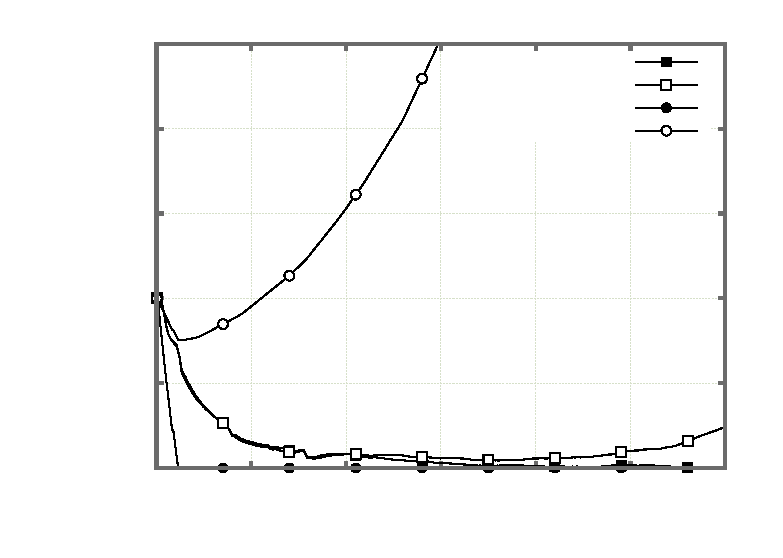
\includegraphics{lower}}%
    \gplfronttext
  \end{picture}%
\endgroup
}
%            \caption{Comparison of dynamics between matrix with side 5 and side
%            25.}
%             \label{fig:lower}
%         \end{minipage}~\hspace*{1em}
%         \begin{minipage}[t]{.6\textwidth}		
%            \vspace{0pt}
%            \centering
%            \resizebox{\columnwidth}{!}{% GNUPLOT: LaTeX picture with Postscript
\begingroup
  \makeatletter
  \providecommand\color[2][]{%
    \GenericError{(gnuplot) \space\space\space\@spaces}{%
      Package color not loaded in conjunction with
      terminal option `colourtext'%
    }{See the gnuplot documentation for explanation.%
    }{Either use 'blacktext' in gnuplot or load the package
      color.sty in LaTeX.}%
    \renewcommand\color[2][]{}%
  }%
  \providecommand\includegraphics[2][]{%
    \GenericError{(gnuplot) \space\space\space\@spaces}{%
      Package graphicx or graphics not loaded%
    }{See the gnuplot documentation for explanation.%
    }{The gnuplot epslatex terminal needs graphicx.sty or graphics.sty.}%
    \renewcommand\includegraphics[2][]{}%
  }%
  \providecommand\rotatebox[2]{#2}%
  \@ifundefined{ifGPcolor}{%
    \newif\ifGPcolor
    \GPcolorfalse
  }{}%
  \@ifundefined{ifGPblacktext}{%
    \newif\ifGPblacktext
    \GPblacktexttrue
  }{}%
  % define a \g@addto@macro without @ in the name:
  \let\gplgaddtomacro\g@addto@macro
  % define empty templates for all commands taking text:
  \gdef\gplbacktext{}%
  \gdef\gplfronttext{}%
  \makeatother
  \ifGPblacktext
    % no textcolor at all
    \def\colorrgb#1{}%
    \def\colorgray#1{}%
  \else
    % gray or color?
    \ifGPcolor
      \def\colorrgb#1{\color[rgb]{#1}}%
      \def\colorgray#1{\color[gray]{#1}}%
      \expandafter\def\csname LTw\endcsname{\color{white}}%
      \expandafter\def\csname LTb\endcsname{\color{black}}%
      \expandafter\def\csname LTa\endcsname{\color{black}}%
      \expandafter\def\csname LT0\endcsname{\color[rgb]{1,0,0}}%
      \expandafter\def\csname LT1\endcsname{\color[rgb]{0,1,0}}%
      \expandafter\def\csname LT2\endcsname{\color[rgb]{0,0,1}}%
      \expandafter\def\csname LT3\endcsname{\color[rgb]{1,0,1}}%
      \expandafter\def\csname LT4\endcsname{\color[rgb]{0,1,1}}%
      \expandafter\def\csname LT5\endcsname{\color[rgb]{1,1,0}}%
      \expandafter\def\csname LT6\endcsname{\color[rgb]{0,0,0}}%
      \expandafter\def\csname LT7\endcsname{\color[rgb]{1,0.3,0}}%
      \expandafter\def\csname LT8\endcsname{\color[rgb]{0.5,0.5,0.5}}%
    \else
      % gray
      \def\colorrgb#1{\color{black}}%
      \def\colorgray#1{\color[gray]{#1}}%
      \expandafter\def\csname LTw\endcsname{\color{white}}%
      \expandafter\def\csname LTb\endcsname{\color{black}}%
      \expandafter\def\csname LTa\endcsname{\color{black}}%
      \expandafter\def\csname LT0\endcsname{\color{black}}%
      \expandafter\def\csname LT1\endcsname{\color{black}}%
      \expandafter\def\csname LT2\endcsname{\color{black}}%
      \expandafter\def\csname LT3\endcsname{\color{black}}%
      \expandafter\def\csname LT4\endcsname{\color{black}}%
      \expandafter\def\csname LT5\endcsname{\color{black}}%
      \expandafter\def\csname LT6\endcsname{\color{black}}%
      \expandafter\def\csname LT7\endcsname{\color{black}}%
      \expandafter\def\csname LT8\endcsname{\color{black}}%
    \fi
  \fi
  \setlength{\unitlength}{0.0500bp}%
  \begin{picture}(7200.00,5040.00)%
    \gplgaddtomacro\gplbacktext{%
      \colorrgb{0.42,0.42,0.42}%
      \put(1210,704){\makebox(0,0)[r]{\strut{} 0}}%
      \colorrgb{0.42,0.42,0.42}%
      \put(1210,1518){\makebox(0,0)[r]{\strut{} 5000}}%
      \colorrgb{0.42,0.42,0.42}%
      \put(1210,2332){\makebox(0,0)[r]{\strut{} 10000}}%
      \colorrgb{0.42,0.42,0.42}%
      \put(1210,3147){\makebox(0,0)[r]{\strut{} 15000}}%
      \colorrgb{0.42,0.42,0.42}%
      \put(1210,3961){\makebox(0,0)[r]{\strut{} 20000}}%
      \colorrgb{0.42,0.42,0.42}%
      \put(1210,4775){\makebox(0,0)[r]{\strut{} 25000}}%
      \colorrgb{0.42,0.42,0.42}%
      \put(1342,484){\makebox(0,0){\strut{} 0}}%
      \colorrgb{0.42,0.42,0.42}%
      \put(2252,484){\makebox(0,0){\strut{} 500}}%
      \colorrgb{0.42,0.42,0.42}%
      \put(3162,484){\makebox(0,0){\strut{} 1000}}%
      \colorrgb{0.42,0.42,0.42}%
      \put(4073,484){\makebox(0,0){\strut{} 1500}}%
      \colorrgb{0.42,0.42,0.42}%
      \put(4983,484){\makebox(0,0){\strut{} 2000}}%
      \colorrgb{0.42,0.42,0.42}%
      \put(5893,484){\makebox(0,0){\strut{} 2500}}%
      \colorrgb{0.42,0.42,0.42}%
      \put(6803,484){\makebox(0,0){\strut{} 3000}}%
      \colorrgb{0.42,0.42,0.42}%
      \put(176,2739){\rotatebox{-270}{\makebox(0,0){\strut{}Living ants}}}%
      \colorrgb{0.42,0.42,0.42}%
      \put(4072,154){\makebox(0,0){\strut{}Time}}%
      \colorrgb{0.42,0.42,0.42}%
      \put(4072,4665){\makebox(0,0){\strut{}}}%
    }%
    \gplgaddtomacro\gplfronttext{%
      \csname LTb\endcsname%
      \put(5804,4602){\makebox(0,0)[r]{\strut{}speedAnts, 100}}%
      \csname LTb\endcsname%
      \put(5804,4382){\makebox(0,0)[r]{\strut{}bruteAnts, 100}}%
      \csname LTb\endcsname%
      \put(5804,4162){\makebox(0,0)[r]{\strut{}speedAnts, 50}}%
      \csname LTb\endcsname%
      \put(5804,3942){\makebox(0,0)[r]{\strut{}bruteAnts, 50}}%
    }%
    \gplbacktext
    \put(0,0){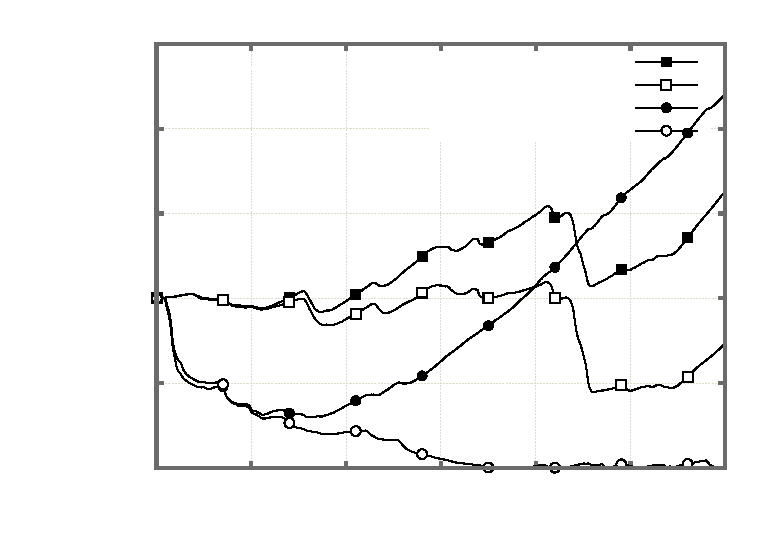
\includegraphics{higher}}%
    \gplfronttext
  \end{picture}%
\endgroup
}
%            \caption{Comparison between matrix with side 50 and side 100}
%            \label{fig:higher}
%         \end{minipage}
%      \end{figure}
      

%      \begin{figure}[H]
%         \centering
%         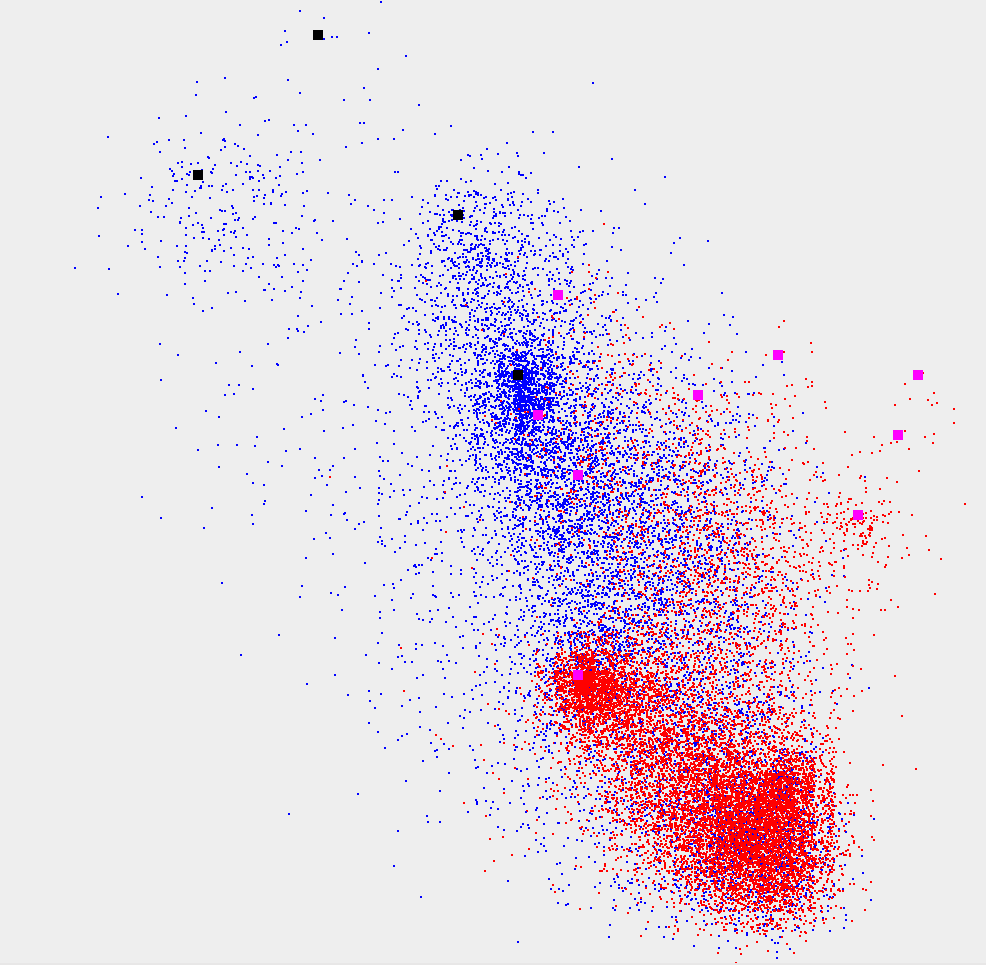
\includegraphics[width=.8\textwidth]{5050foodhunt.png}
%         \caption{Snapshot of simulation in a $50 \times 50$ matrix.
%            \texttt{speedAnts} are represented with blue dots (black anthills), while
%            \texttt{bruteAnts} are seen as red (magenta anthills). In this capture, ants are seen
%            having just finished a source of food, and are returning homeward.} 
%         \label{fig:graph}            
%      \end{figure}


\newpage

\begin{thebibliography}{99}
   \bibitem{lecnotes}
     Tobias Ambjörnsson,
     \emph{Lecture notes, Computational Physics},
     Department of Astronomy and Theoretical Physics,
     Lund University,
     2015.
  \bibitem{midges}
      A. Attanasi et al,
      \emph{Collective Behaviour without Collective Order in Wild Swarms of
      Midges},
      PLoS Computational Biology: 10(7),
      2014.
   \bibitem{ants}
      D. Jin et al,
      \emph{Ant Colony Optimization with a new Random Walk Model for Community
      Detection in Complex Networks},
      Jilin University,
      2013.
\end{thebibliography}
\newpage
\appendix
\section{Code}
 %  \label{sec:code}
 %  \lstinputlisting[language=Java]{Common.java}
 %  \lstinputlisting[language=Java]{Forest.java}
 %  \lstinputlisting[language=Java]{Square.java}
 %  \lstinputlisting[language=Java]{Food.java}
 %  \lstinputlisting[language=Java]{Anthill.java}
 %  \lstinputlisting[language=Java]{AntPanel.java}
 %  \lstinputlisting[language=Java]{Ant.java}
 %  \lstinputlisting[language=Java]{SpeedAnt.java}
 %  \lstinputlisting[language=Java]{BruteAnt.java}
\end{document}

